\documentclass[11pt,a4paper]{article}
% ── Typography ────────────────────────────────────────────────────────────────
\usepackage[margin=2.5cm]{geometry}
\usepackage[utf8]{inputenc}
\usepackage[T1]{fontenc}
\usepackage{lmodern}
\usepackage{microtype}
% ── Colour, Graphics ─────────────────────────────────────────────────────────
\usepackage{xcolor}
\usepackage{tikz}
\usetikzlibrary{shapes.geometric, arrows.meta, positioning, fit, backgrounds,
                decorations.pathreplacing, calc, shadows.blur}
% ── Tables ───────────────────────────────────────────────────────────────────
\usepackage{booktabs}
\usepackage{array}
\usepackage{colortbl}
\usepackage{multirow}
% ── Document ─────────────────────────────────────────────────────────────────
\usepackage{listings}
\usepackage{hyperref}
\usepackage{enumitem}
\usepackage{fancyhdr}
\usepackage{amsmath}
\usepackage{amssymb}

% ── Colour palette ────────────────────────────────────────────────────────────
\definecolor{fpgablue}{RGB}{13,71,161}
\definecolor{fpgalight}{RGB}{187,222,251}
\definecolor{fpgamid}{RGB}{100,160,220}
\definecolor{hostgreen}{RGB}{27,94,32}
\definecolor{hostlight}{RGB}{200,230,201}
\definecolor{ibkrorange}{RGB}{200,80,0}
\definecolor{ibkrlight}{RGB}{255,224,178}
\definecolor{sigred}{RGB}{183,28,28}
\definecolor{codegray}{RGB}{248,248,248}
\definecolor{arrowgray}{RGB}{80,80,80}
\definecolor{sectionbg}{RGB}{232,240,254}
\definecolor{noteblue}{RGB}{227,242,253}
\definecolor{noteborder}{RGB}{100,160,220}

% ── TikZ styles ───────────────────────────────────────────────────────────────
\tikzset{
  block/.style={rectangle, rounded corners=4pt, minimum width=2.6cm,
    minimum height=1cm, text centered, draw, font=\small\bfseries,
    text width=2.4cm},
  fpgablock/.style={block, fill=fpgalight, draw=fpgablue, text=fpgablue},
  hostblock/.style={block, fill=hostlight, draw=hostgreen, text=hostgreen},
  ibkrblock/.style={block, fill=ibkrlight, draw=ibkrorange, text=ibkrorange},
  arrow/.style={-{Stealth[length=6pt]}, thick, color=arrowgray},
  fatarrow/.style={-{Stealth[length=8pt]}, line width=2pt, color=fpgablue},
  slowarrow/.style={-{Stealth[length=8pt]}, line width=2pt, color=ibkrorange},
}

% ── Page style ────────────────────────────────────────────────────────────────
\pagestyle{fancy}
\fancyhf{}
\rhead{\small\textcolor{fpgablue}{FPGA Tick-to-Trade}}
\lhead{\small Why FPGAs Beat CPUs: Parallelism}
\cfoot{\small\thepage}
\renewcommand{\headrulewidth}{0.5pt}

\hypersetup{colorlinks=true, linkcolor=fpgablue, urlcolor=fpgablue,
            pdftitle={Why FPGAs Beat CPUs --- Parallelism, DSP Wiring, and Multi-Core}}

\lstset{
  backgroundcolor=\color{codegray}, basicstyle=\ttfamily\small,
  keywordstyle=\color{fpgablue}\bfseries, commentstyle=\color{gray}\itshape,
  stringstyle=\color{sigred}, breaklines=true, frame=single,
  rulecolor=\color{gray!40}, numbers=left, numberstyle=\tiny\color{gray},
  xleftmargin=1.5em, xrightmargin=0.5em, language=Verilog,
}

% ── Note box helper ───────────────────────────────────────────────────────────
\newenvironment{notebox}{%
  \begin{center}
  \begin{tikzpicture}
  \node[rectangle, rounded corners=4pt, fill=noteblue, draw=noteborder,
        text width=13cm, inner sep=10pt, font=\small]
  \bgroup\begin{minipage}{13cm}}%
  {\end{minipage}\egroup;
  \end{tikzpicture}
  \end{center}}

\title{\vspace{-1cm}\textcolor{fpgablue}{\Large\bfseries Why FPGAs Beat CPUs for Tick-to-Trade}\\[4pt]
       \large Parallelism, DSP Wiring, and the Multi-Core Question}
\author{\small FPGA-Accelerated HFT Project}
\date{\small 2026-06-12}

\begin{document}
\maketitle
\thispagestyle{fancy}

\begin{notebox}
\textbf{The core idea.} On a CPU, ``steps'' happen one after another \emph{in time}
on a shared engine. On an FPGA, ``steps'' are physical circuits laid out \emph{in
space}, and they all run \emph{every clock cycle at once}. For a short, fixed,
latency-critical pipeline like tick-to-trade, that difference is decisive --- and,
crucially, deterministic.
\end{notebox}

% ══════════════════════════════════════════════════════════════════════════════
\section{Two Flavours of FPGA Parallelism}

Before comparing against CPUs, it is worth separating the two distinct things people
mean by ``the FPGA runs in parallel.''

\subsection*{1. Spatial parallelism (within one cycle)}

Consider the imbalance comparison, expressed without division via the
cross-multiplication identity $a/b > k \iff a\cdot k_d > k_n \cdot b$:
\[
  \texttt{bid\_size} \times 10 \;>\; 15 \times \texttt{ask\_size}.
\]
On a CPU this is two multiplies and a compare --- three sequential instructions sharing
one ALU. On the FPGA there are \textbf{two physical DSP multiplier blocks sitting side
by side on the die}. One computes $\texttt{bid\_size}\times 10$, the other computes
$15\times\texttt{ask\_size}$, \emph{at the same time}, because they are different lumps
of silicon. Their outputs feed a comparator. Everything resolves within a
\textbf{single clock cycle}.

\begin{center}
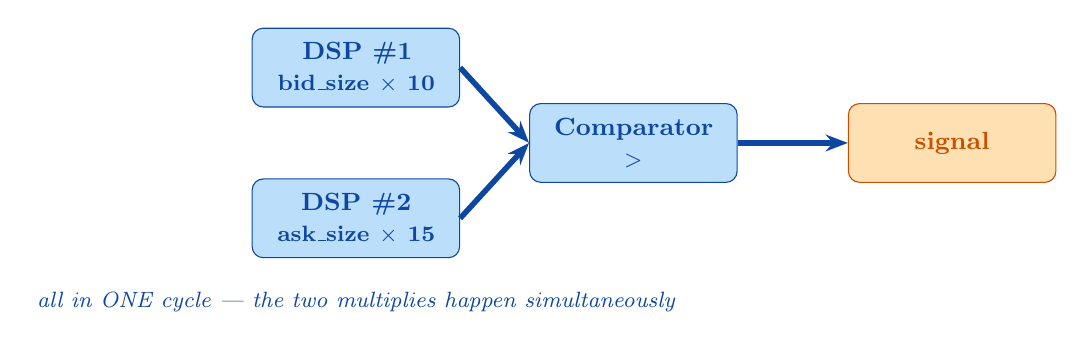
\begin{tikzpicture}[node distance=0.9cm and 1.4cm]
  \node[fpgablock] (m1) {DSP \#1\\ \footnotesize bid\_size $\times$ 10};
  \node[fpgablock, below=of m1] (m2) {DSP \#2\\ \footnotesize ask\_size $\times$ 15};
  \node[fpgablock, right=2.2cm of $(m1)!0.5!(m2)$] (cmp) {Comparator\\ \footnotesize $>$};
  \node[ibkrblock, right=of cmp] (sig) {signal};
  \draw[fatarrow] (m1.east) -- (cmp.west);
  \draw[fatarrow] (m2.east) -- (cmp.west);
  \draw[fatarrow] (cmp.east) -- (sig.west);
  \node[font=\footnotesize\itshape, below=0.3cm of m2, text=fpgablue]
        {all in ONE cycle --- the two multiplies happen simultaneously};
\end{tikzpicture}
\end{center}

\subsection*{2. Pipeline parallelism (across cycles)}

Each stage of the tick-to-trade path is its own circuit with a register at its output.
On \textbf{every clock cycle}, all stages are active --- each working on a
\emph{different message}.

\begin{center}
\begin{tabular}{l|ccccc}
\toprule
\textbf{cycle} $\rightarrow$ & 1 & 2 & 3 & 4 & 5 \\
\midrule
Stage A: parse type     & msg1 & msg2 & msg3 & msg4 & msg5 \\
Stage B: shift fields    & ---  & msg1 & msg2 & msg3 & msg4 \\
Stage C: update book     & ---  & ---  & msg1 & msg2 & msg3 \\
Stage D: compute signal  & ---  & ---  & ---  & msg1 & msg2 \\
\bottomrule
\end{tabular}
\end{center}

By cycle 4 the pipeline is full: Stage A parses msg4 while Stage D computes the signal
for msg1 --- \emph{all four in the same cycle}. A CPU has one engine, so it can only be
``in'' one stage at a time.

% ══════════════════════════════════════════════════════════════════════════════
\section{What ``DSP Wiring'' Means}

\textbf{DSP = Digital Signal Processing block} --- a small, hardened, pre-built
multiply--accumulate circuit baked into the FPGA silicon. On the Xilinx VU9P (the AWS F1
chip) these are \textbf{DSP48E2 slices}, and there are about \textbf{6{,}840} of them
scattered across the die. Each can compute, in one cycle:
\[
  \texttt{result} = (A + D)\times B + C,
\]
a multiplier feeding an adder/accumulator with optional I/O registers. It is not
``programmed'' like a CPU instruction --- it is a physical block of optimised transistors
that does multiply--add and nothing else.

\textbf{Wiring it} means: in your RTL, when you write

\begin{lstlisting}
wire [47:0] left  = bid_size * 16'd10;   // synthesizes to DSP #1
wire [47:0] right = ask_size * 16'd15;   // synthesizes to DSP #2
wire signal = (left > right);            // synthesizes to LUT comparator
\end{lstlisting}

the synthesis tool \textbf{maps} each multiply onto a physical DSP block. The ``wires''
are the actual metal routing carrying \texttt{bid\_size}'s bits \emph{into} DSP \#1's
input port and its 48-bit output \emph{out} toward the comparator. You are literally
describing which silicon blocks connect to which.

\begin{notebox}
\textbf{Temporal vs. spatial.} On a CPU, \texttt{bid\_size * 10} is a \emph{temporal}
event --- an instruction that occupies the one ALU for some cycles. On the FPGA it is a
\emph{spatial} fact --- a specific block at specific die coordinates, always there,
always wired the same way.
\end{notebox}

% ══════════════════════════════════════════════════════════════════════════════
\section{``But CPUs Have Many Cores'' --- The Three Reasons}

Multi-core is real parallelism, but it is a \textbf{coarse, expensive} kind that does not
help the \emph{small} operations on a tick-to-trade path. Three reasons.

\subsection*{Reason 1 --- Core count vs. operation count}

\begin{center}
\renewcommand{\arraystretch}{1.3}
\begin{tabular}{>{\bfseries}l c c}
\toprule
 & \textbf{CPU core} & \textbf{FPGA LUT / DSP} \\
\midrule
Count          & 32--64                    & $\sim$1.2M LUTs / $\sim$6{,}840 DSPs \\
Does           & \emph{any} instruction, one at a time & \emph{one} fixed tiny op, always \\
Parallel unit  & a whole thread            & a single gate / multiply \\
\bottomrule
\end{tabular}
\end{center}

A CPU core is a heavyweight generalist. To run your two multiplies ``in parallel'' on two
cores, each core still fetches, decodes, and executes --- hundreds of cycles of overhead
to parallelize an operation the FPGA does in \emph{one} cycle with zero overhead.

\subsection*{Reason 2 --- The unit of parallelism is too big}

Cores parallelize at the granularity of \textbf{threads} --- chunks of work big enough to
justify the cost of coordination. Splitting $\texttt{bid\_size}\times 10$ and
$\texttt{ask\_size}\times 15$ across two cores is absurd: the work is nanoseconds, but
launching/syncing threads costs \textbf{microseconds}. You would lose by orders of
magnitude. FPGA parallelism is at the granularity of \textbf{a single arithmetic
operation, or even a single bit} --- no thread, no scheduler, no coordination cost. That
is exactly the scale this problem lives at.

\subsection*{Reason 3 --- Cores still share memory and are not deterministic}

Even if you did spread work across cores, they share:
\begin{itemize}[leftmargin=1.4em, itemsep=2pt]
  \item \textbf{The cache hierarchy} --- one core's miss stalls it $\sim$100+ cycles, unpredictably.
  \item \textbf{The memory bus} --- contention between cores adds jitter.
  \item \textbf{Coherency traffic} --- keeping caches in sync between cores costs cycles, non-deterministically.
  \item \textbf{The OS scheduler} --- it can migrate or preempt your thread at any moment.
\end{itemize}
Multi-core gives more \emph{throughput} for big independent jobs (rendering, compiling,
serving many requests), but does \textbf{nothing} for the \emph{latency} of one small
dependent chain like \texttt{parse $\rightarrow$ update $\rightarrow$ compare}.

\subsection*{Side by side}

\begin{center}
\begin{tikzpicture}[node distance=0.7cm]
  % CPU side
  \node[ibkrblock, minimum width=3.2cm] (cpu) {CPU (even 64 cores)};
  \node[font=\footnotesize, below=0.2cm of cpu, text width=5.8cm, align=center]
    {realistically runs on \textbf{one} core, sequentially:\\
     {[mul]}{[mul]}{[cmp]} $+$ risk of cache miss / preempt.\\
     Splitting across cores costs \textmu s to save ns.};
  % FPGA side
  \node[fpgablock, minimum width=3.2cm, right=5.5cm of cpu] (fpga) {FPGA};
  \node[font=\footnotesize, below=0.2cm of fpga, text width=5.8cm, align=center]
    {DSP\#1: bid$\times$10 \;\textbar\; DSP\#2: ask$\times$15\\
     $\rightarrow$ comparator $\rightarrow$ signal,\\
     \textbf{all in ONE cycle, every cycle, forever.}};
\end{tikzpicture}
\end{center}

% ══════════════════════════════════════════════════════════════════════════════
\section{The Real Distinction}

It is not ``FPGA has more parallelism than a multi-core CPU.'' It is that they
parallelize at \textbf{different granularities}:

\begin{itemize}[leftmargin=1.4em, itemsep=4pt]
  \item \textbf{CPU cores:} a \emph{few} generalist engines, parallel at the
  \textbf{thread} level. Great for many big independent tasks. Overhead too high for tiny
  ops; shared resources kill determinism.
  \item \textbf{FPGA:} \emph{millions} of tiny specialist circuits, parallel at the
  \textbf{operation/bit} level. Each does one fixed thing every cycle. Perfect for a
  short, fixed, latency-critical pipeline.
\end{itemize}

For HFT the bottleneck is \textbf{the latency of one message through one short chain}, not
the throughput of millions of independent jobs. Multi-core attacks the wrong axis; the
FPGA attacks exactly yours --- and does it deterministically:
\[
  p99 = p50 = p1.
\]

\begin{notebox}
\textbf{Bottom line.} The slowest message and the median message take \emph{identically}
long. No cache to miss, no branch to mispredict, no OS to interrupt. For tick-to-trade,
predictable worst-case latency is worth more than raw average speed --- and that is
something cores fundamentally cannot promise.
\end{notebox}

\end{document}
